\setchapterpreamble[u]{
    \dictum[Master Yoda en \textit{Return of the Jedi}]{\raggedleft\textquote{Always pass on what you have learned.}}
}
\chapter{Tecnologías y metodologías usadas}
% Se ha intentado usar herramientas gratuitas basadas en software libre para evitar el coste de compra de licencias.
% permitir que cualquiera pueda replicar los resultados del proyecto.
% y gratuito debido a que el proyecto no cuenta con ningún presupuesto más allá de los recursos humanos.
% No obstante, se han usado herramientas de diseño no-libres como QuestaSim y Xilinx Vivado, pues ya se disponía de una licencia de uso en el departamento. 
% Aunque se hubiese preferido usar íntegramente herramientas libres, se ha optado por el uso de las que habíamos usado en proyectos anteriores (en asignaturas como Tecnología y Organización de Computadores), debido a la falta de tiempo y recursos para el descubrimiento y aprendizaje de nuevas herramientas.

% En las herramientas, debido al poco tiempo del proyecto se han usado principalmente herramientas conocidas y usadas previamente durante la carrera, como Xilinx Vivado, también porque el departamento disponía de licencias de uso.
En las herramientas, se han usado principalmente herramientas compatibles con las FPGAs que posee el grupo de investigación, fabricadas por Xilinx, el mayor fabricante de FPGAs.

Por otro lado, se han utilizado lenguajes de scripting como \textit{Python}, \textit{Bash}, \textit{Perl} o \textit{TCL} para la realización de distintas tareas. El uso de algunas de las herramientas se ha realizado mediante una conexión por escritorio remoto a una máquina Windows con las herramientas preinstaladas, debido a los altos requisitos del sistema para la ejecución de este tipo de aplicaciones.

En las siguientes secciones se detallan las herramientas más usadas en el proyecto.

\section{Redacción y documentación}

\subsection{Overleaf y \LaTeX}

Para la redacción de la memoria de este proyecto se ha usado el sistema de preparación de documentos \LaTeX. Un lenguaje de marcado en el que se intercala redacción en texto plano con macros que especifican su formato.

Para hacer posible la colaboración entre los integrantes del proyecto (estudiante y directores) se ha usado Overleaf, un editor colaborativo alojado en la nube que usa el conjunto de paquetes de LaTeX ``TeXlive" para proporcionar un entorno completo de elaboración de documentos sin necesidad de instalar nada.

\begin{figure}[h]
    \centering
    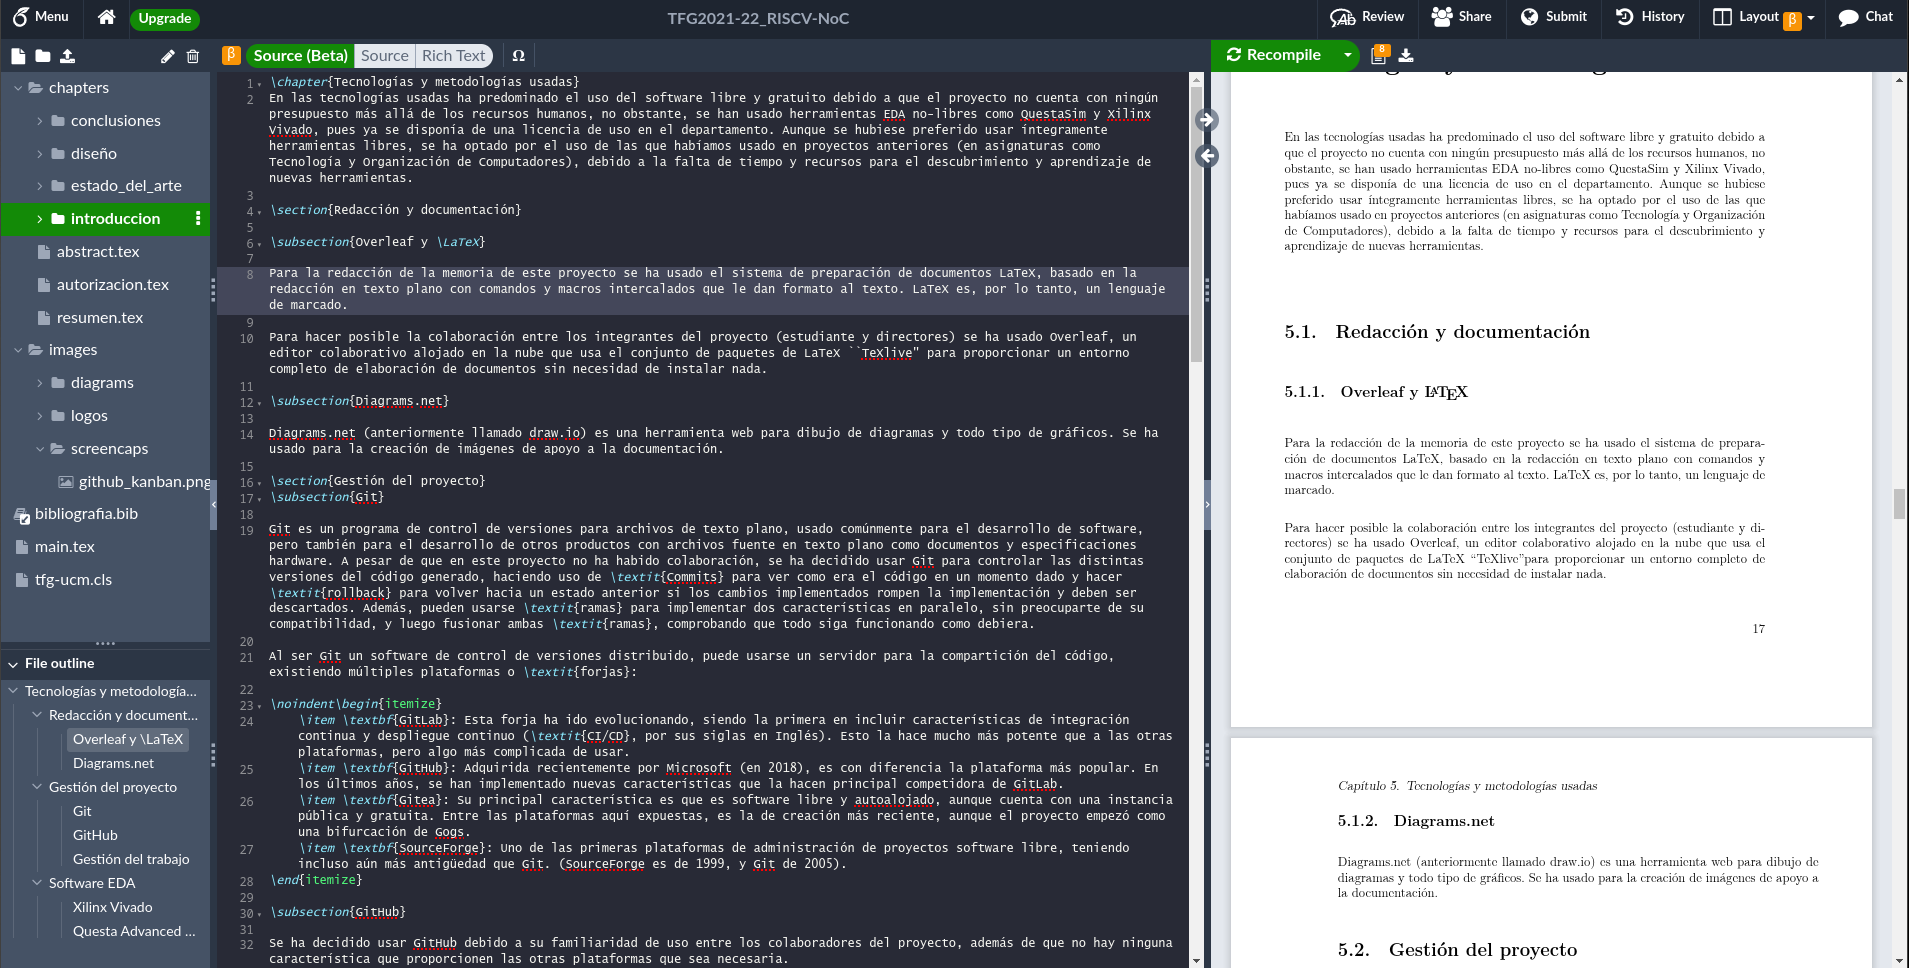
\includegraphics[width=\linewidth]{images/screencaps/overleaf.png}
    \caption{Captura de pantalla del proyecto de la memoria en Overleaf}
    \label{fig:screencap_overleaf}
\end{figure}

Para la creación de diagramas e imágenes de apoyo a la documentación se ha usado diagrams.net (anteriormente llamado draw.io), una herramienta web para el dibujo de todo tipo de gráficos.

\section{Gestión del proyecto}
\subsection{Git}

Git es un programa de control de versiones para archivos de texto plano, usado comúnmente para el desarrollo de software, pero también para el desarrollo de otros productos con archivos fuente en texto plano como documentos y especificaciones hardware. A pesar de que en este proyecto no ha habido colaboración, se ha decidido usar Git para controlar las distintas versiones del código generado, haciendo uso de \textit{Commits} para poder visualizar las diferencias en el código a lo largo del tiempo y hacer \textit{rollback} para volver hacia un estado anterior si los cambios implementados rompen el correcto funcionamiento del proyecto y deben ser descartados. Además, pueden usarse \textit{ramas} para implementar dos características en paralelo, sin preocuparte de su compatibilidad, y luego fusionar ambas \textit{ramas}, comprobando que todo siga funcionando como debiera.

% \noindent\begin{itemize}
%     \item \textbf{GitLab}: Esta forja ha ido evolucionando, siendo la primera en incluir características de integración continua y despliegue continuo (\textit{CI/CD}, por sus siglas en Inglés). Esto la hace mucho más potente que a las otras plataformas, pero algo más complicada de usar.
%     \item \textbf{GitHub}: Adquirida recientemente por Microsoft (en 2018), es con diferencia la plataforma más popular. En los últimos años, se han implementado nuevas características que la hacen principal competidora de GitLab.
%     \item \textbf{Gitea}: Su principal característica es que es software libre y autoalojado, aunque cuenta con una instancia pública y gratuita. Entre las plataformas aquí expuestas, es la de creación más reciente, aunque el proyecto empezó como una bifurcación de Gogs.
%     \item \textbf{SourceForge}: Uno de las primeras plataformas de administración de proyectos software libre, teniendo incluso aún más antigüedad que Git. (SourceForge es de 1999, y Git de 2005).
% \end{itemize}

\subsubsection{GitHub}

Al ser Git un software de control de versiones distribuido, puede usarse un servidor para la compartición del código, existiendo múltiples plataformas o \textit{forjas}. Además de compartir código, la mayoría de forjas tienen una interfaz web en la que se dan herramientas para facilitar la colaboración. De entre ellas, se ha elegido \textbf{GitHub} debido a la familiaridad de uso entre los colaboradores del proyecto. En los últimos años han implementado diversas características y mejoras a la gestión de proyectos, haciendo que, además de alojar el código, pueda llevarse a cabo la dirección del proyecto y asignación de tareas desde una única plataforma.

% Se ha decidido usar GitHub debido a su familiaridad de uso entre los colaboradores del proyecto, además de que no hay ninguna característica que proporcionen las otras plataformas que sea necesaria.

Se han creado múltiples repositorios para manejar mejor las distintas partes diferenciadas del proyecto.

\begin{itemize}
    \item \textbf{\href{https://github.com/daviddavo/Cores-SweRV-EL2-NoC}{daviddavo/Cores-SweRV-EL2-NoC}}: Un \textit{fork} o ramificación del repositorio del SweRV-EL2 de chipsalliance. En este repositorio se han realizado los cambios tanto en el diseño como en el sistema de compilación para incluir la NoC en la unidad de ejecución.
    \item \textbf{\href{https://github.com/daviddavo/tfg_poc_noc}{daviddavo/tfg\_poc\_noc}}: Se incluye el código del diseño y herramientas para la compilación de la NoC de manera aislada.
    \item \textbf{\href{https://github.com/ogarnica/TFG2021-22_RISC-V_NoC}{ogarnica/TFG2021-22\_RISC-V\_NoC}}: Proyecto principal. Cuenta con los otros dos proyectos instalados como \textit{submódulos}, de tal manera que al descargar este proyecto se descargan también los otros dos. Entre los archivos del proyecto también se encuentra documentación técnica, el código \LaTeX  de esta memoria, los datos usados en el procesamiento de datos para los gráficos de la memoria, y el sistema de issues y kanban usados para la gestión del proyecto.
\end{itemize}

\subsection{Gestión del trabajo}

Para la gestión de tareas se ha usado un tablero \textit{Kanban}, en el que cada tarea está representada por una tarjeta que se va moviendo entre las diversas columnas dependiendo de su grado de completitud. Cada una de las tarjetas permite hacer un seguimiento exhaustivo de la tarea que representa, pudiendo ser etiquetada, asignada a una persona, y comentada. En nuestro caso, el tablero cuenta con las siguientes columnas:

\begin{itemize}
    \item \textbf{\textit{To do}}: Se incluyen todas las tareas por hacer o a considerar, pueden no estar asignadas a nadie aún.
    \item \textbf{\textit{Sprint}}: Tareas por hacer, pero con un plazo de entrega próximo. Son tareas que reciben una especial prioridad y deben completarse lo antes posible.
    \item \textbf{\textit{Blocked}}: Tareas bloqueadas a la espera de que acabe algún otro proceso. Pueden estar bloqueadas por otra tarea del proyecto, o por una causa externa (por ejemplo, esperar a que la licencia de un software se renueve).
    \item \textbf{\textit{In progress}}: Tareas que se están realizando ahora mismo. En la filosofía Kanban es muy importante poner un límite al número de tareas que puede manejar un solo usuario, y poder visualizar en todo momento las tareas que se estan realizando actualmente.
    \item \textbf{\textit{Review}}: Tareas terminadas que deben ser revisadas. En este caso, por los directores del proyecto.
    \item \textbf{\textit{Done}}: Esta columna sirve de registro de todas las tareas que han sido terminadas.
\end{itemize}

Este tablero ha sido alojado también en GitHub, permitiéndonos hacer referencias al código fácilmente y trabajar con las ramas de git.

\begin{figure}[h]
    \centering
    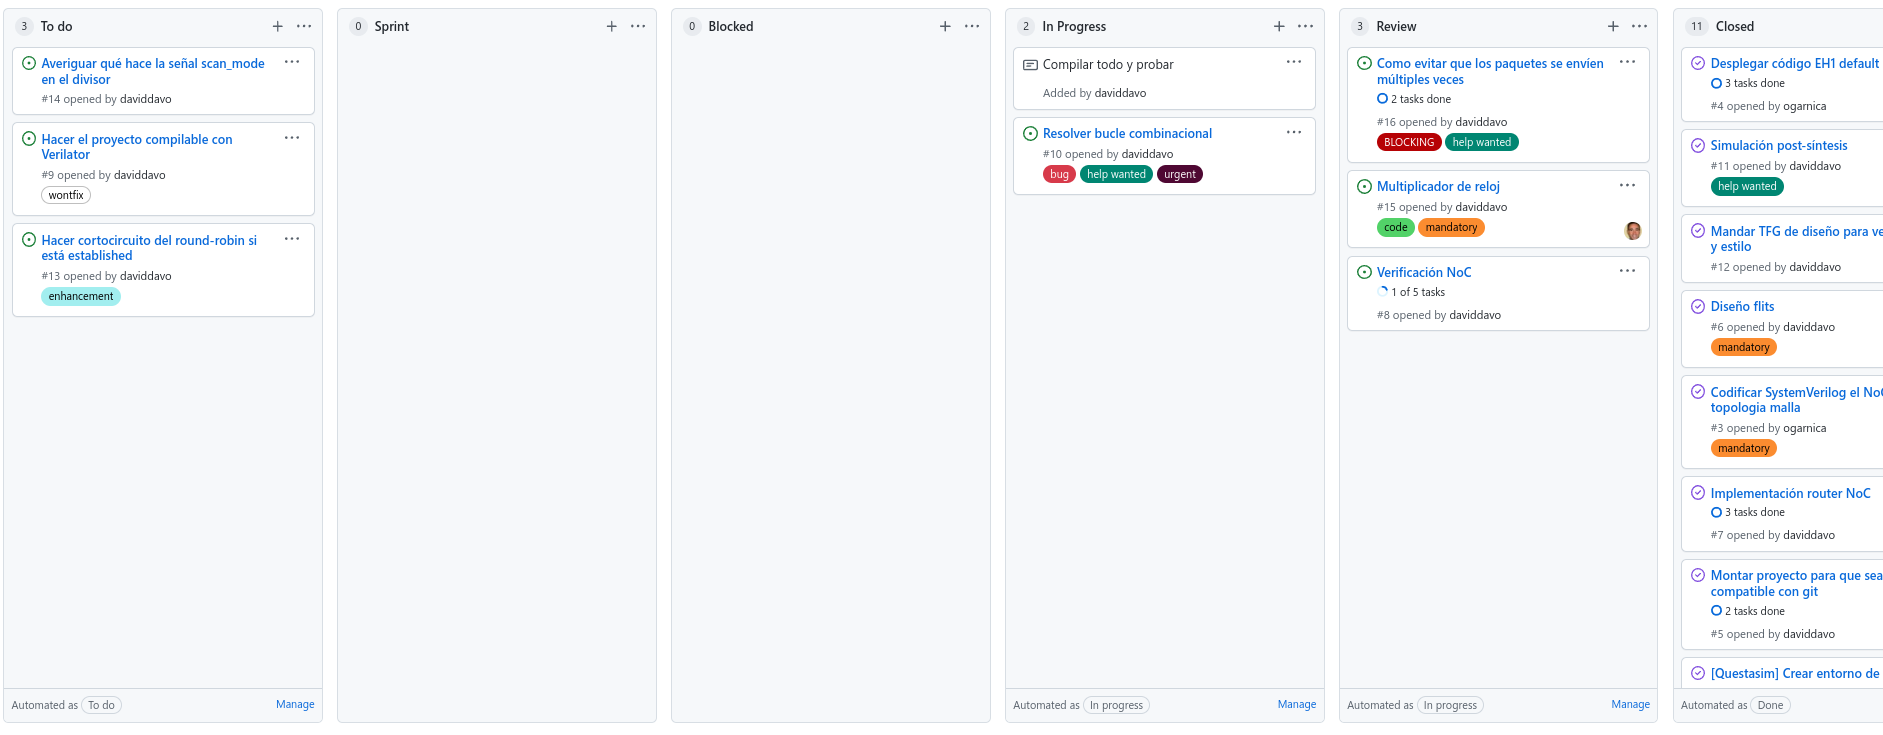
\includegraphics[width=\linewidth]{images/screencaps/github_kanban.png}
    \caption{Captura de pantalla del tablero Kanban de GitHub en la fase tardía del desarrollo del proyecto}
    \label{fig:screencap_kanban}
\end{figure}

\section{Diseño hardware}

El software \textit{Electronic Design Automation} (EDA) o de Diseño Electrónico Automático, también llamado \textit{Electronic Computer-Aided Design} (ECAD) o de Diseño Electrónico Asistido por Computadora, sigue un flujo de diseño para la descripción, elaboración y análisis de circuitos integrados.

Por lo general, el flujo de trabajo es el siguiente (resumido en la figura \ref{fig:diagram_design_flow}):
\begin{itemize}
    \item \textbf{Diseño}: Se escribe en algún lenguaje de descripción de hardware (como SystemVerilog o VHDL) el diseño, creando una representación del circuito en alto nivel conocida como RTL (\textit{Register-Transfer Level}). En el RTL se modelan los registros y las operaciones lógicas de las señales que circulan entre ellos.
    Antes de continuar, debemos ejecutar una simulación de este modelo, creando un \textit{testbench} para verificar si el diseño cumple con las funcionalidades requeridas (también llamada simulación \textit{conductual} o de \textit{comportamiento}).
    % Se hace síntesis de alto nivel, convirtiendo la descripción en Verilog/VHDL a un modelo ejecutable en el PC en, por ejemplo, C/C++. Este modelo \textit{conductual} permite verificar rápidamente el diseño ejecutando un \textit{testbench}. Este proceso también se conoce como elaboración o síntesis a nivel de transferencia de registros (RTL o \textit{Register-Transfer Level}).
    \item \textbf{Síntesis}: Es un proceso en el que se traduce el RTL a una \textit{netlist}: una descripción que representa las puertas lógicas o registros utilizados y las conexiones entre ellos. 
    % Podemos ejecutar simulaciones más precisas si añadimos cierto retardo simulado a cada uno de los nodos (puertas) y vértices (pistas o cables) del grafo. 
    También se generan reportes con estimaciones temporales y de consumo, y de problemas combinacionales que puedan surgir (por ejemplo, si el circuito tiene bucles combinacionales, o se puede calcular el camino más largo posible que restringirá nuestro ciclo de reloj). 
    Finalmente, podemos realizar una simulación post-síntesis en la que se añade cierto retardo aproximado a cada una de las puertas y conexiones, comprobando que el funcionamiento sigue siendo el esperado.
    \item \textbf{Implementación}: Se optimiza el \textit{netlist} generado en el punto anterior y se asigna a cada elemento de la \textit{netlist} una de las primitivas de la FPGA (\textit{map}), por ejemplo, para implementar una función lógica se usarán varios LUTs distintos, pero sin tener en cuenta su ubicación en la FPGA. En el \textit{place \& route} se coloca cada uno de los elementos de la netlist en un elemento físico de la FPGA, intentando cumplir las restricciones temporales establecidas. Finalmente, se traduce esta información a un binario que configurará la FPGA (\textit{bitstream}). En este moneto ya podemos estimar con precisión el tiempo que tardarán las operaciones combinacionales, su consumo, o incluso la temperatura alcanzable por las áreas de la FPGA. Con herramientas más avanzadas puede comprobarse que los campos electromagnéticos generados por las señales no generarán problemas como \textit{crosstalk}, o simularse la lógica a nivel de transistor en caso de querer fabricar el circuito.
\end{itemize}

\begin{figure}[h]
    \centering
    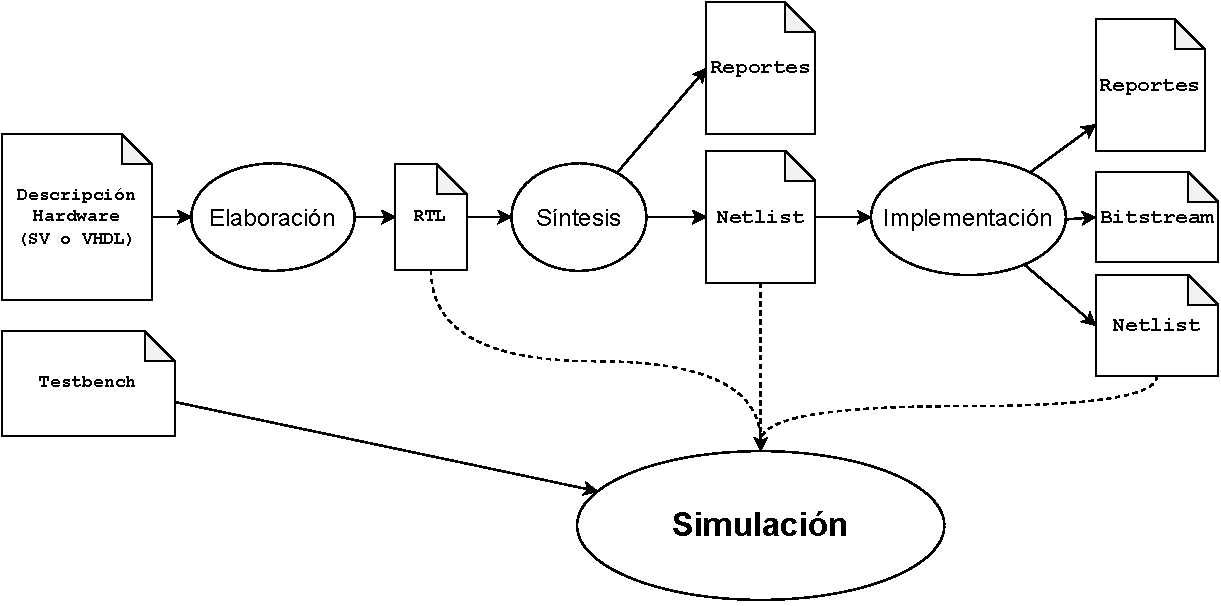
\includegraphics[width=\textwidth]{images/diagrams/design_flow.drawio.pdf}
    % \missingfigure{Incluir figura con el flujo de diseño y los productos generados en cada fase (que se pasan a la siguiente)}
    \caption{Representación del flujo de diseño hardware.}
    \label{fig:diagram_design_flow}
\end{figure}

En este proyecto nos hemos enfocado en la fase de diseño RTL, pero creando código que sea \textit{sintetizable} para que pueda ser usado en una FPGA si es preciso.

\subsection{FPGA}
Una Matriz Programable de Puertas Lógicas o FPGA (\textit{Field-Programmable Gate Array}) es un dispositivo diseñado para permitir que el usuario configure la matriz de puertas lógicas de tal manera que pueda formarse un circuito.

La FPGA contiene bloques lógicos configurables (CLBs) que, conectados y configurados correctamente, nos permiten crear cualquier circuito lógico. Cada CLB cuenta con varios elementos, como registros o \textit{flip-flops} y tablas de verdad o LUTs (\textit{LookUp-Tables}), que permiten especificar cualquier función lógica (normalmente, de un número reducido de entradas, 3 o 4 bits). Algunos CLBs pueden incluir funciones lógicas más complicadas pero muy usadas, como sumadores o multiplexores. Aun así, algunas FPGA incluyen elementos fuera de los CLBs accesibles por nuestro circuito, como son memorias de acceso aleatorio en bloque (BRAM), procesadores de señales digitales (DSP)  o interfaces de comunicación avanzadas (Ethernet, PCIe).

También es posible reconfigurar tan solo partes de la FPGA, permitiéndonos modificar parte del diseño en tiempo de ejecución,
añadiendo, modificando, quitando, intercambiando o reubicando módulos cuando sea necesario; por ejemplo, si un diseño es demasiado grande puede dividirse en submódulos que se van llevando a la FPGA según se van necesitando. Además, esta característica puede aprovecharse para crear diseños tolerantes a fallos: en caso de que la radiación electromagnética degrade el sustrato en el que se sitúa un submódulo, este puede reimplementarse en un área libre de la FPGA para que el dispositivo siga funcionando correctamente.
%añadir y quitar características en tiempo de ejecución conforme va siendo necesario, o reprogramar partes que se vayan degradando con el tiempo, por ejemplo por radiación electromagnética de alta energía en aplicaciones espaciales.

\subsection{Xilinx Vivado}

Vivado es el software EDA elegido para el diseño y la síntesis de la NoC. La versión utilizada es la 2021.2, con la licencia WebPACK Edition, sin coste pero con una cantidad disponible de dispositivos objetivo reducida.
% Se ha usado el lenguaje de descripción de hardware SystemVerilog (superset de Verilog) para el diseño y la simulación. 
Se ha elegido Vivado pues al estar creado por Xilinx, la misma compañía que produce la FPGA elegida, tiene una gran compatibilidad con esta. Además, no ha sido necesario aprender su uso al haberse usado anteriormente en otras asignaturas del grado.

Es capaz de mostrar los diagramas de bloques del RTL generados, muy útil para la depuración y solución de los errores detectados durante la síntesis y simulación. También pueden generarse multitud de reportes, presentando los recursos consumidos por nuestro diseño en potencia y área de la FPGA, o señalando violaciones de las restricciones temporales especificadas para las señales de nuestro diseño (por ejemplo, si un reloj tiene demasiada latencia puede hacer que se desincronice la lógica secuencial).

Sin embargo, el simulador integrado en Vivado no cuenta con demasiadas características y no es muy potente, por lo que se ha optado por usar un simulador externo.

\begin{figure}[h]
    \centering
    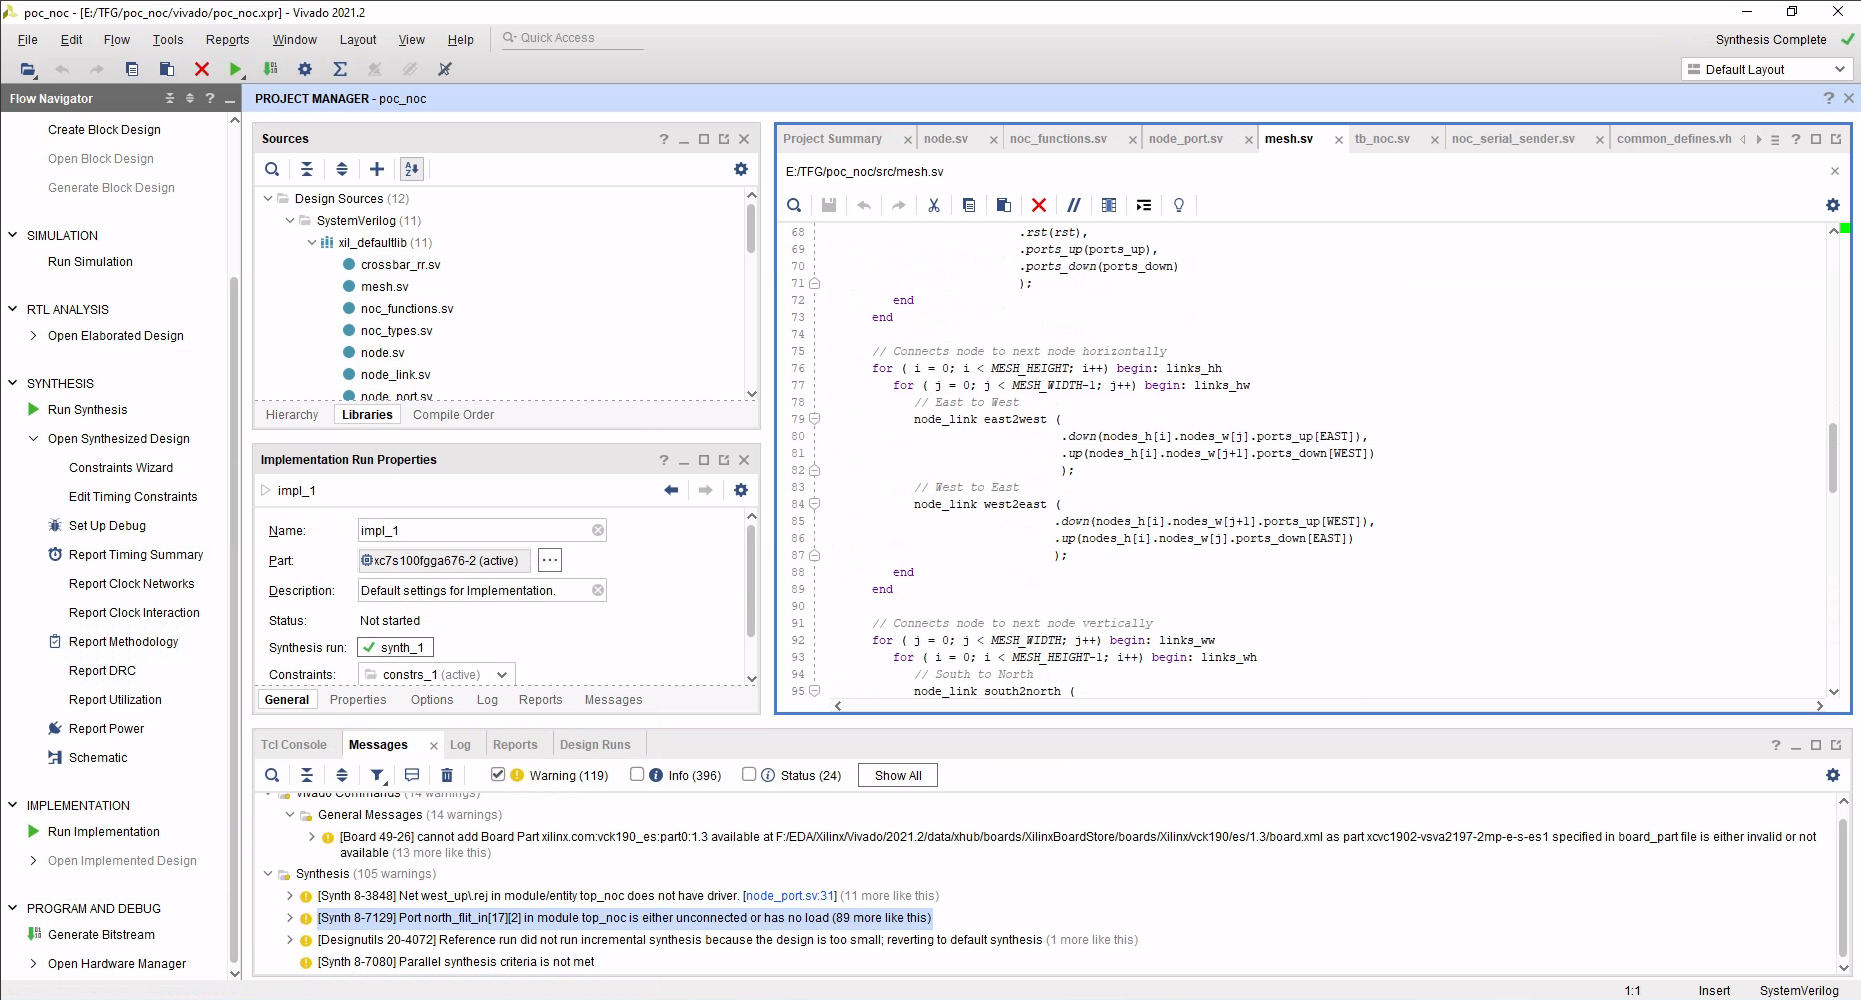
\includegraphics[width=\linewidth]{images/screencaps/vivado.png}
    \caption{Captura de pantalla de Xilinx Vivado 2021.2 en su vista de edición de código}
    \label{fig:screencap_vivado}
\end{figure}

\subsection{Questa Advanced Simulator}

QuestaSim es un entorno gráfico de verificación, simulación y depuración de lenguajes de descripción de hardware de Siemens EDA\footnote{La productora original del simulador es Mentor Graphics, adquirida en 2017 por Siemens}.
Actualmente en el proyecto se utiliza la versión 2022.1. Se ha usado para simular y depurar los diseños RTL y los sintetizados por Vivado.

Cuenta tanto con un entorno por línea de comandos para realizar pruebas \textit{por lotes} no supervisadas (pudiendo exportar los resultados de las formas de onda), como con una interfaz gráfica en la que es posible mostrar un diagrama de tiempos con las formas de onda de las señales de nuestro diseño, tanto de entrada/salida como internas.

Puede integrarse con Vivado para ejecutar fácilmente simulaciones post-síntesis utilizando las librerías de simulación de los elementos básicos de la FPGA, incluyendo los retardos de cada una de las señales y puertas lógicas.

\begin{figure}[h]
    \centering
    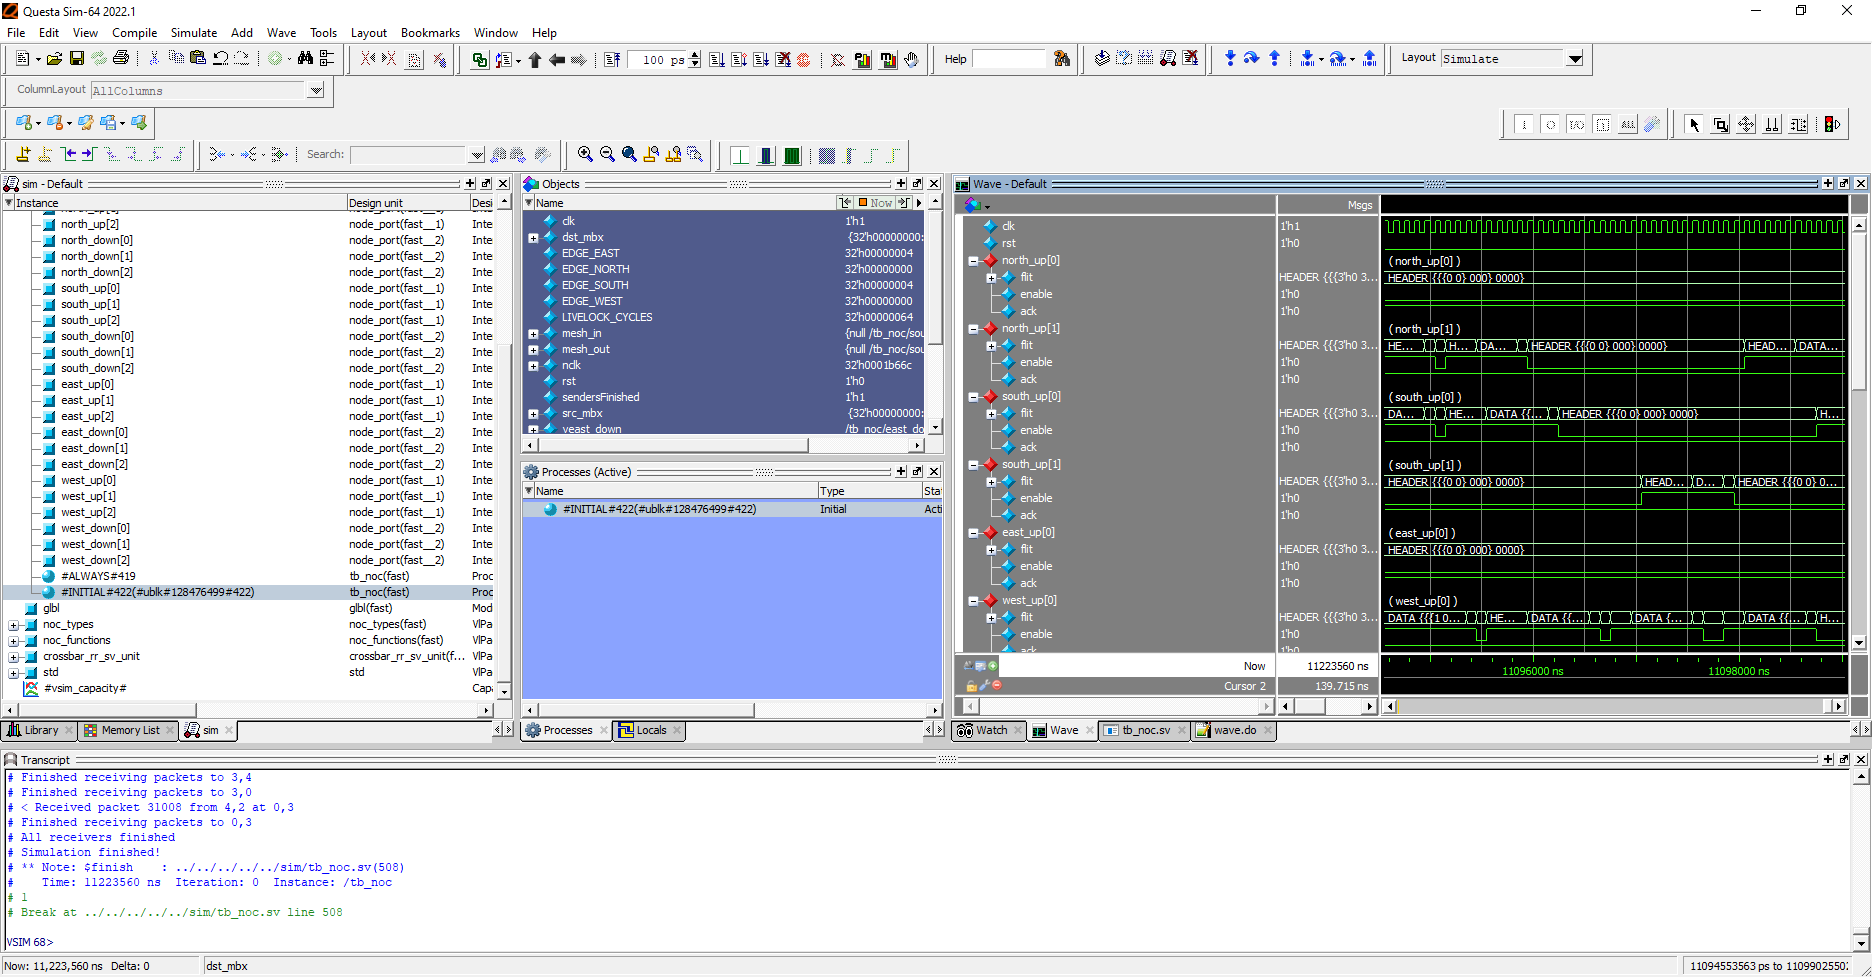
\includegraphics[width=\linewidth]{images/screencaps/questasim.png}
    \caption{Captura de pantalla de QuestaSim 2022.1 tras ejecutar una simulación de la NoC.}
    \label{fig:screencap_questasim}
\end{figure}